\section{Hardware specification}
The platform selected needs to fulfill the requirements set in the theory section, and will be a hub where different sensors such as a camera and distance sensor can be mounted and integrated. The following section describes the hardware specification of the complete system.
\subsection{Raspberry Pi 3 Model B}
The Raspberry Pi, developed in the United Kingdom by the Raspberry Pi Foundation, is the single-board computer selected for my application. It is a powerful computer and has the I/O peripheral support expected from a regular PC. It features a powerful processing unit suited for image processing, and enough RAM to support such applications. The Raspberry Pi is open source and compatible with many operating systems, opening up for further improvement by other project- and master students.\\

Specifications\cite{rpi}:
\begin{itemize}
\itemsep0em 
\item \textbf{System-on-chip} Broadcom BCM2837
\item \textbf{CPU} 1.2 GHz 64-bit quad-core ARM Cortex-A53
\item \textbf{Memory} 1 GB LPDDR2 RAM at 900 MHz
\item \textbf{Graphics}	Broadcom VideoCore IV 400 MHz
\item \textbf{Power} 10.0 W (2 A)
\end{itemize}
\begin{figure}[H]
  \centering
  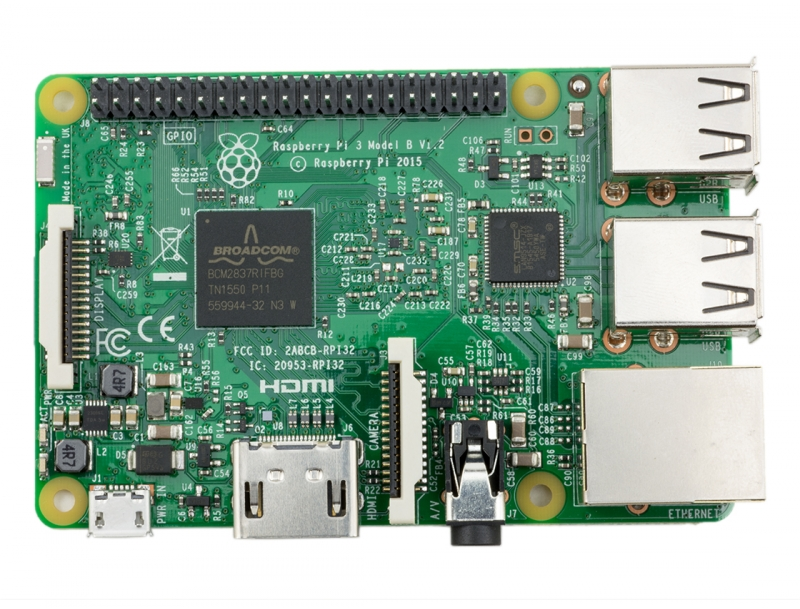
\includegraphics[width=0.6\textwidth]{fig/rpi}
  \caption{Raspberry Pi 3 Model B}
  \label{fig:gsd}
\end{figure}

Other technical specifications\cite{rpi}:
\begin{itemize}
\itemsep0em 
\item Bluetooth Low Energy (BLE)
\item BCM43438 WiFi
\item 40pin extended GPIO
\item 4 x USB 2 ports
\item 4 pole Stereo output and Composite video port
\item Full size HDMI output
\item CSI camera port for connecting the Raspberry Pi camera
\item DSI display port for connecting the Raspberry Pi touch screen display
\item Micro SD port for loading operating system and storing data
\end{itemize}


\subsection{Raspberry Pi Camera Module v2}
The Raspberry Pi Camera Module v2 is the second version of the camera module produced by the Raspberry Pi Foundation. It features excellent compatibility with the Raspberry Pi, and is open-source. %Litt mer
\begin{figure}[H]
  \centering
  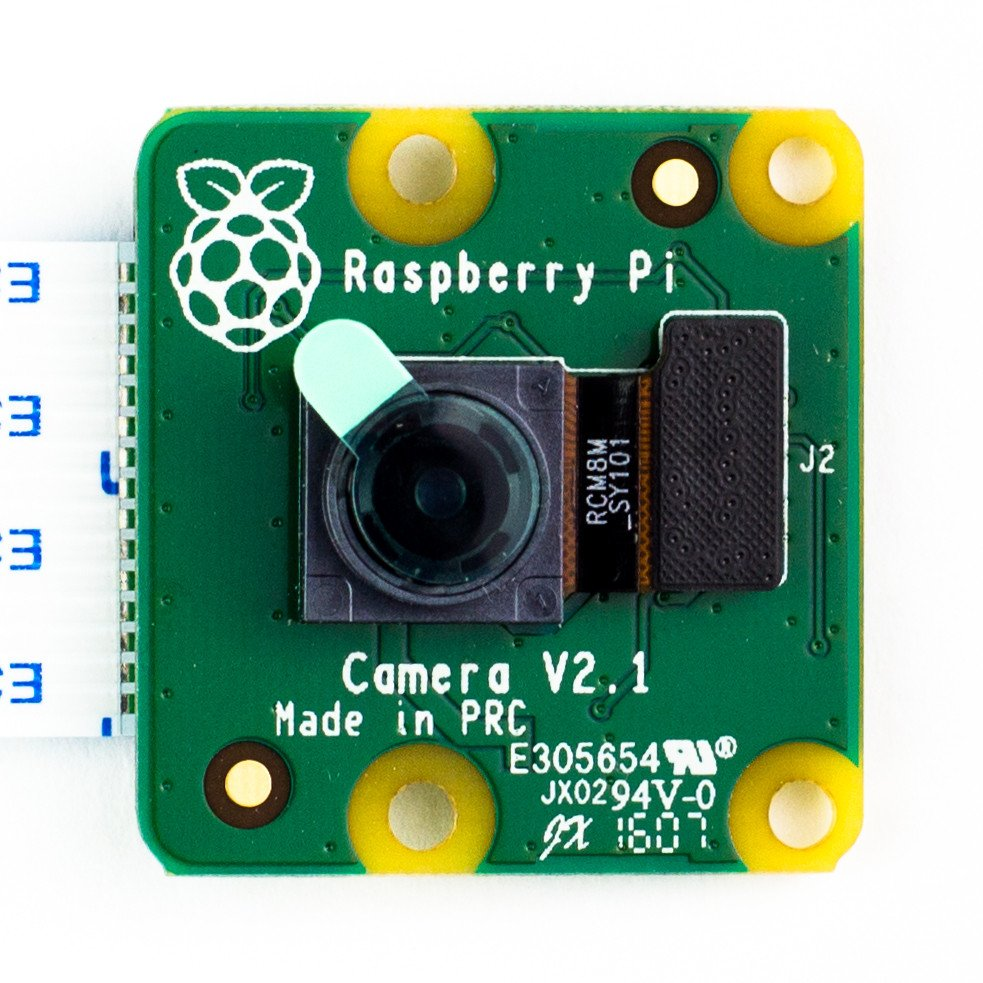
\includegraphics[width=0.4\textwidth]{fig/picam}
  \caption{Raspberry Pi Camera Module v2}
  \label{fig:picam}
\end{figure}

Specifications\cite{cam}:
\begin{itemize}
\itemsep0em
\item \textbf{Sensor} Sony IMX219
\item \textbf{Sensor Resolution} 3280$\times$ 2464 pixels
\item \textbf{Sensor Image Area} 3.68$\times$ 2.76 mm (4.6mm diagonal)
\item \textbf{Pixel Size} 1.12 $\mu m$ $\times$ 1.12 $\mu m$
\item \textbf{Focal length} 3.04 mm
\end{itemize}
%skrive mer

\subsection{HC - SR04 Ultrasonic Ranging Module}
\begin{figure}[H]
  \centering
  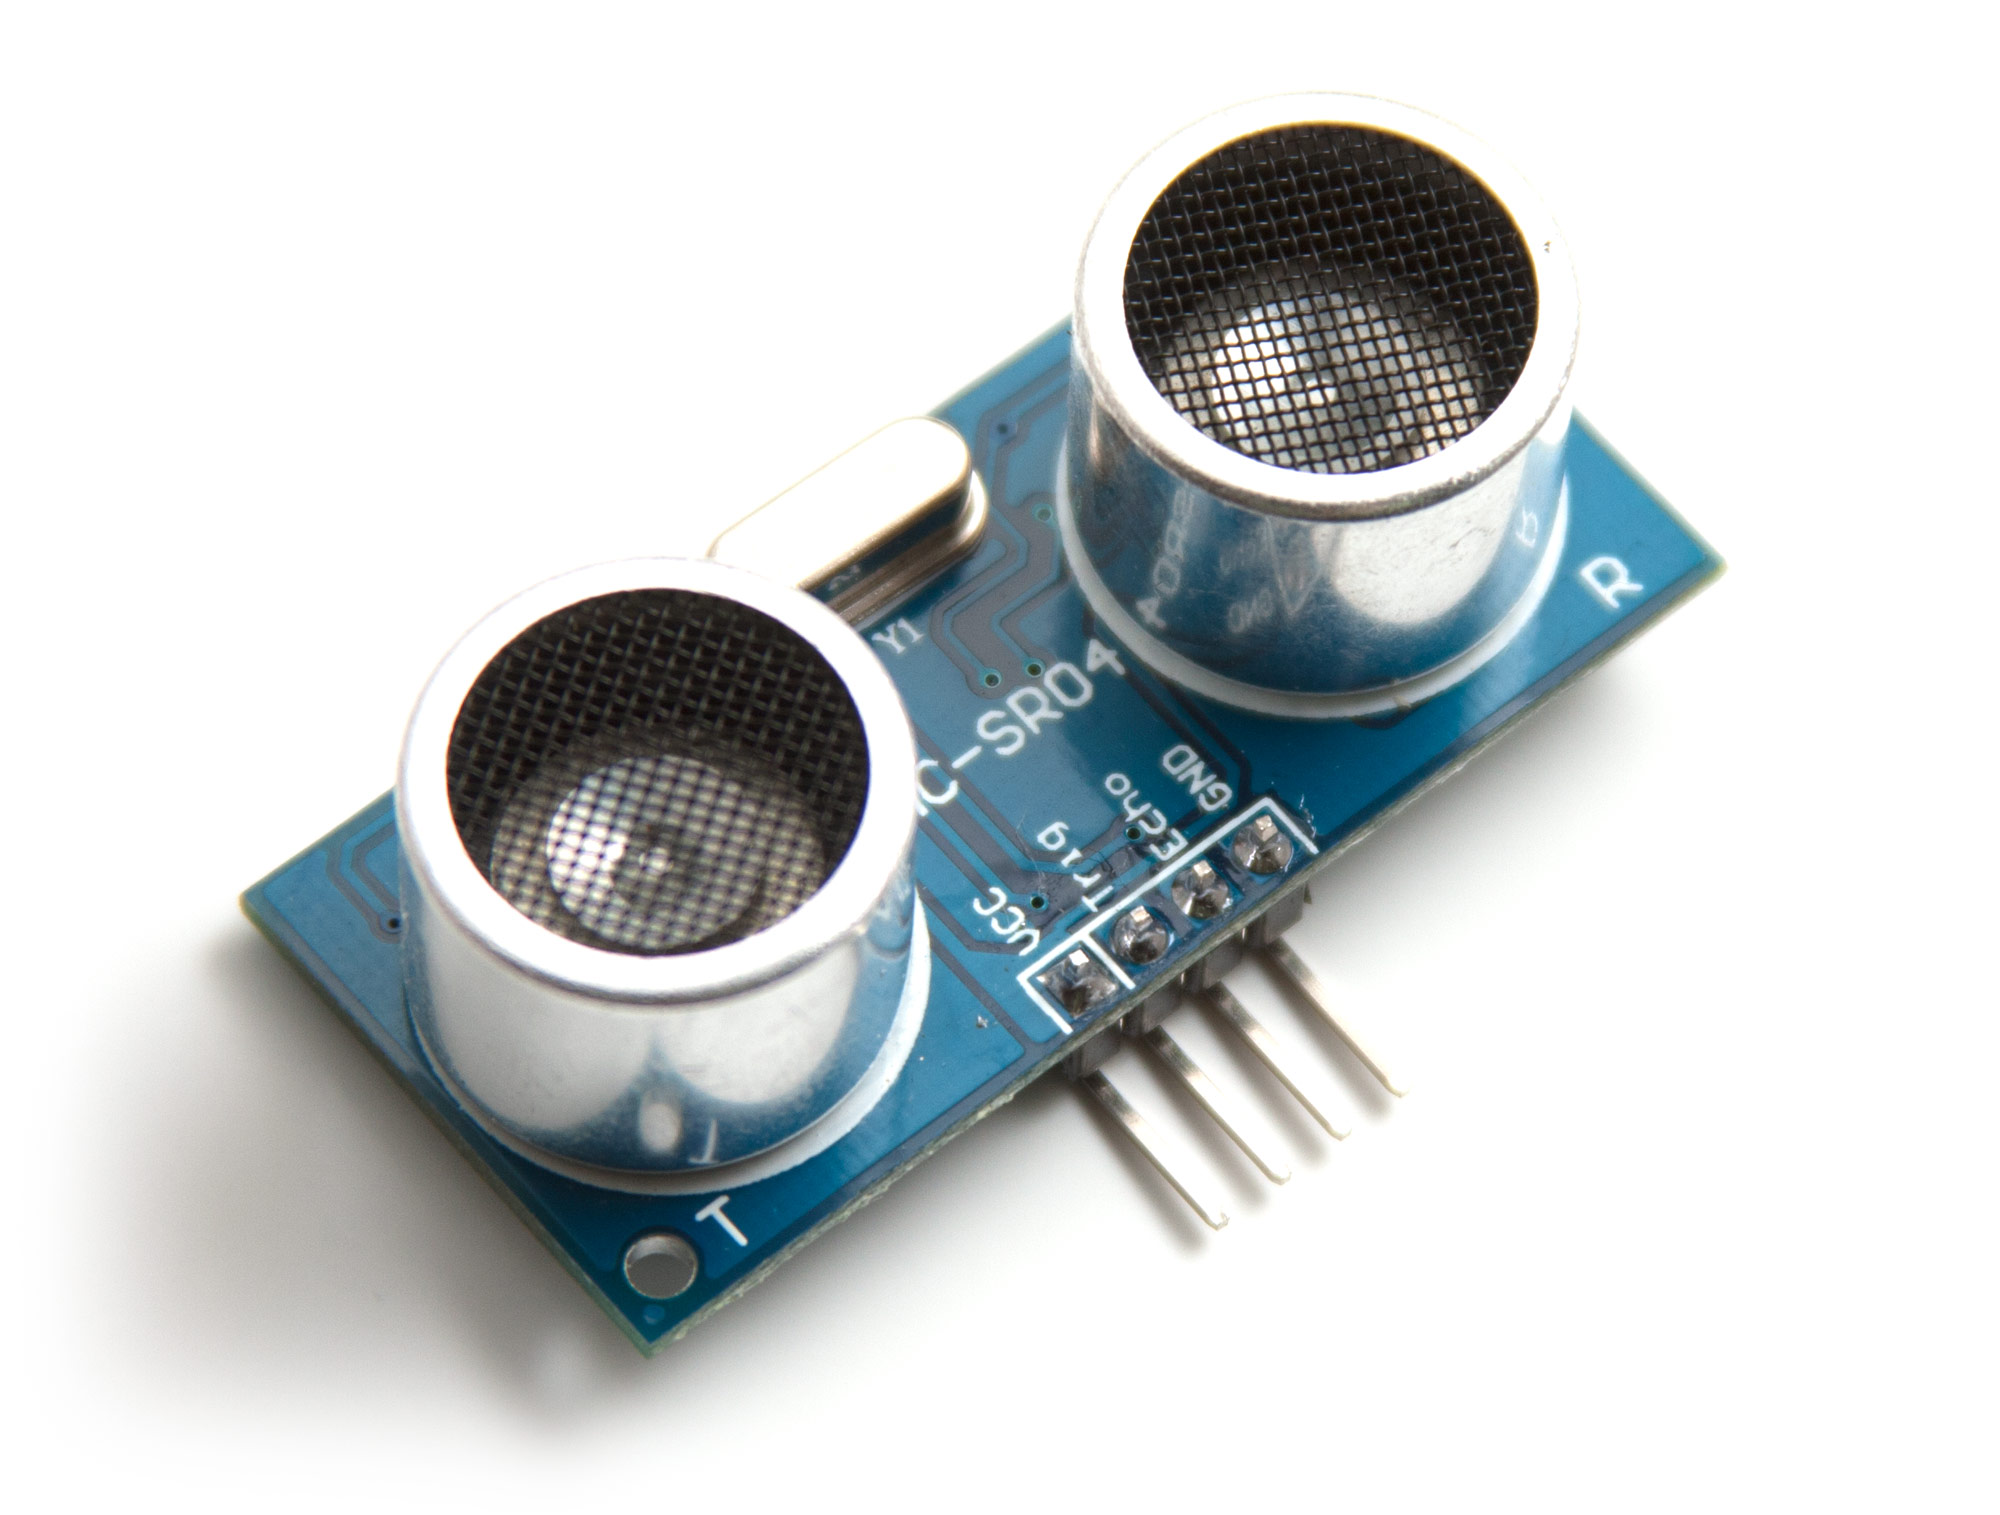
\includegraphics[width=0.3\textwidth]{fig/hc}
  \caption{HC - SR04}
  \label{fig:hc}
\end{figure}
\begin{itemize}
\itemsep0em
\item \textbf{Max Range} 4 m
\item \textbf{Min Range} 2 cm
\item \textbf{Resolution} 0.3 cm
\item \textbf{Working Voltage} DC 5V
\end{itemize}

The HC - SR04 is an ultrasonic range sensor made by Cytron Technologies. It features a range interval suitable for the application in this project, and has a good resolution for a low price. It is compatible with the Raspberry Pi, and has a track record of usage in Raspberry Pi projects.

\subsection{Raspberry Pi Universal Power Supply}
\begin{figure}[H]
  \centering
  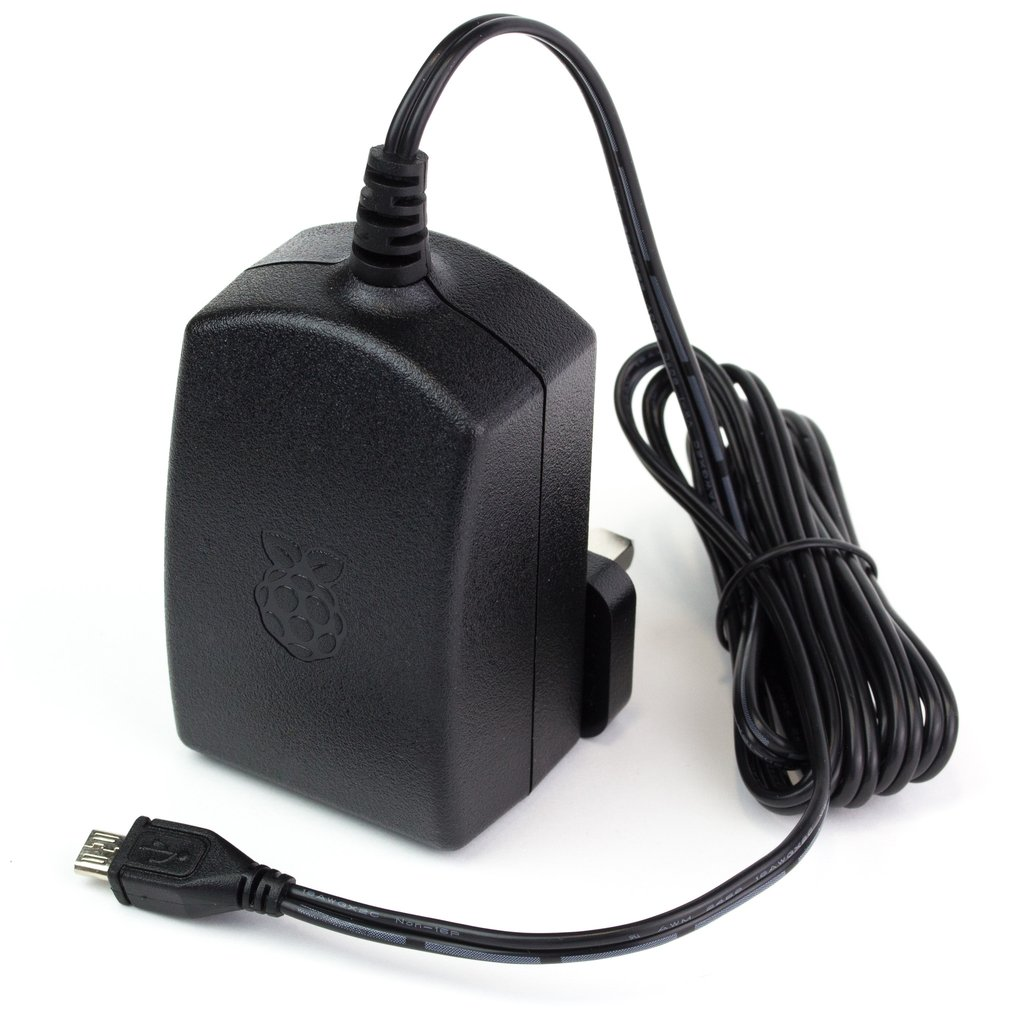
\includegraphics[width=0.3\textwidth]{fig/rpipower}
  \caption{Raspberry Pi Universal Power Supply}
  \label{fig:power}
\end{figure}
\begin{itemize}
\itemsep0em 
\item \textbf{Input:} 100-240V
\item \textbf{Output:} 5.1V/2.5A
\end{itemize}
This power supply is the official Raspberry Pi model.








